\documentclass{beamer} % [notes=only]
\usetheme{Intel}

\setbeamertemplate{section in toc}{\inserttocsectionnumber.~\inserttocsection} % Use number keys for table of content sections.
\setbeamertemplate{subsection in toc}{\hspace{0.5cm}\rule[0.3ex]{3pt}{3pt}~\inserttocsubsection\par} % Use a symbol for table of content subsections.
\AtBeginSection[]
{
	\begin{frame}
		\frametitle{Table of Contents}
		\tableofcontents[currentsection]
    \end{frame}
} % Insert table of contents frame before each new section.
\setbeamertemplate{caption}[numbered] % Number figures.

\definecolor{intel}{RGB}{0, 113, 197}
\setbeamercolor{section in toc shaded}{fg=intel}
\setbeamercolor{subsection in toc shaded}{fg=black}
\setbeamercolor{section in toc}{fg=intel}
\setbeamercolor{subsection in toc}{fg=black}
\setbeamercolor{block title}{fg=intel}
\setbeamercolor{caption name}{fg=intel}

\usepackage{hyperref}
\usepackage{multicol} % Used to split up table of contents in a double column style.
\usepackage{multirow} % Needed for multirow graphs
\usepackage{datetime} % Used to format dates.
\usepackage{listings} % Used to format inline code throughout document.
\usepackage{color} % Used to gray out text
\usepackage{tikz} % Used to gain access to the \centering command.
\usepackage[mediumspace,mediumqspace,squaren,binary]{SIunits} % \milli\second
\usepackage{keystroke} % Used for key icons.

\hypersetup{
	colorlinks=false,
	linkcolor=blue,
	urlcolor=black,
	citecolor=blue,
	anchorcolor=blue
}
\usetikzlibrary{calc}

\newenvironment{graytext}{\color{gray}}{\ignorespacesafterend}

\newcommand{\mascfirstline}[1]{\input{#1}\unskip}

\lstset{
	language=C,
	tabsize=4,
	backgroundcolor=\color{black!5},
	basicstyle=\tiny,
}

\newcommand{\dvtcmdcodeinline}[1]{
	\colorbox{black!5}{
			\lstinline[basicstyle=\ttfamily\color{black}]{#1}}}

\newtheorem{thm}{Key point}

\begin{document}
	\title{Paravirtualizing OpenGL ES in Simics}
\subtitle{Master's Thesis in Computer Science}
\author{Eric Nilsson}
\institute{Intel Corporation}
\date{\today}

\begin{frame}
	\titlepage
\end{frame}


	\section{Introduction}

	\subsection{Simics}
	\input{simics.tex}

        \subsection{Terminology}
        \begin{frame}
\frametitle{Paravirtualization}

Brief slide on paravirtualization and what we mean by it

\end{frame}

        \begin{frame}
\frametitle{Hardware-assisted virtualization}

\begin{itemize}
	\item Simics relies on interpretation and JIT to accelerate simulation
	\item To further speed-up simulation, Simics can utilize hardware-assisted virtualization on those processors that support it
	\item This requires that the simulated platform corresponds to the host platform
\end{itemize}

\end{frame}


	\subsection{Question formulation}
	\begin{frame}
\frametitle{Key points}

\begin{block}{\#1}
	Paravirtualization is a viable method of accelerating graphics
\end{block}

\begin{block}{\#2}
	Magic instructions is a suitable communications medium
\end{block}

\begin{block}{\#3}
	The case for paravirtualization is strengthened for systems where hardware-assisted virtualization is unavailable
\end{block}

\end{frame}


        \subsection{Background}
        \begin{frame}
\frametitle{Background}

\begin{itemize}
\item Virtual platforms are key to reducing Time-to-Market
\item Improved simulation performance enables more use-cases
\item Because of architectural differences, GPU workloads are sub-optimal for CPUs
\item Therefore, some method of accelerating graphics in Simics is desireable
\end{itemize}

\begin{center}
{\Huge $\hookleftarrow$}
\end{center}

\end{frame}

        \begin{frame}
\frametitle{User example - Tracing}

An example of why paravirtualization in Simics is of interest

\end{frame}


	\subsection{Graphics simulation}
	\begin{frame}
\frametitle{Graphics simulation}

\begin{columns}
	\column{0.5\textwidth}
	\begin{block}{GPU modeling}
		Modeling the GPU ISA
                \begin{itemize}
                  \item Costly
                  \item Performance obstacles
                \end{itemize}
	\end{block}
	\begin{block}{PCI passthrough}
		First-hand device access using passthrough technologies
                \begin{itemize}
                  \item Requires dedicated hardware\phantom{     }
                  \item Difficult to implement robust checkpointing
                \end{itemize}
	\end{block}
    \column{0.5\textwidth}
    \begin{block}{Soft modeling}
    	Software rasterization
        \begin{itemize}
        \item Easy but often good-enough
        \item Performance obstacles
        \end{itemize}
    \end{block}
    \begin{block}{Paravirtualization}
    	Selectively modify virtual architecture
        \begin{itemize}
          \item Facilitate checkpointing in software
          \item Cost-effective but possibly heavy maintenence
        \end{itemize}
    \end{block}
\end{columns}
	
\end{frame}


        \section{Methodology and experiment}

        \subsection{Summary}
	\begin{frame}
  \frametitle{Summary}

  \begin{block}{Method}
    \begin{itemize}
    \item Paravirtualized graphics in Simics
    \item Accelerates OpenGL ES 2.0
    \end{itemize}
  \end{block}

  \begin{block}{Evaluation}
    \begin{itemize}
    \item Run benchmarks stressing suspected optimal and sub-optimal use-case
    \item Compare performance to software rasterization
    \end{itemize}
  \end{block}

  \begin{block}{Conclusion}
    \begin{itemize}
    \item Performance improvements (up to $34$ times)
    \item Located bottleneck
    \end{itemize}
  \end{block}

\end{frame}


	\subsection{Simics pipe}
	\begin{frame}
\frametitle{Simics Pipe}

\begin{center}
	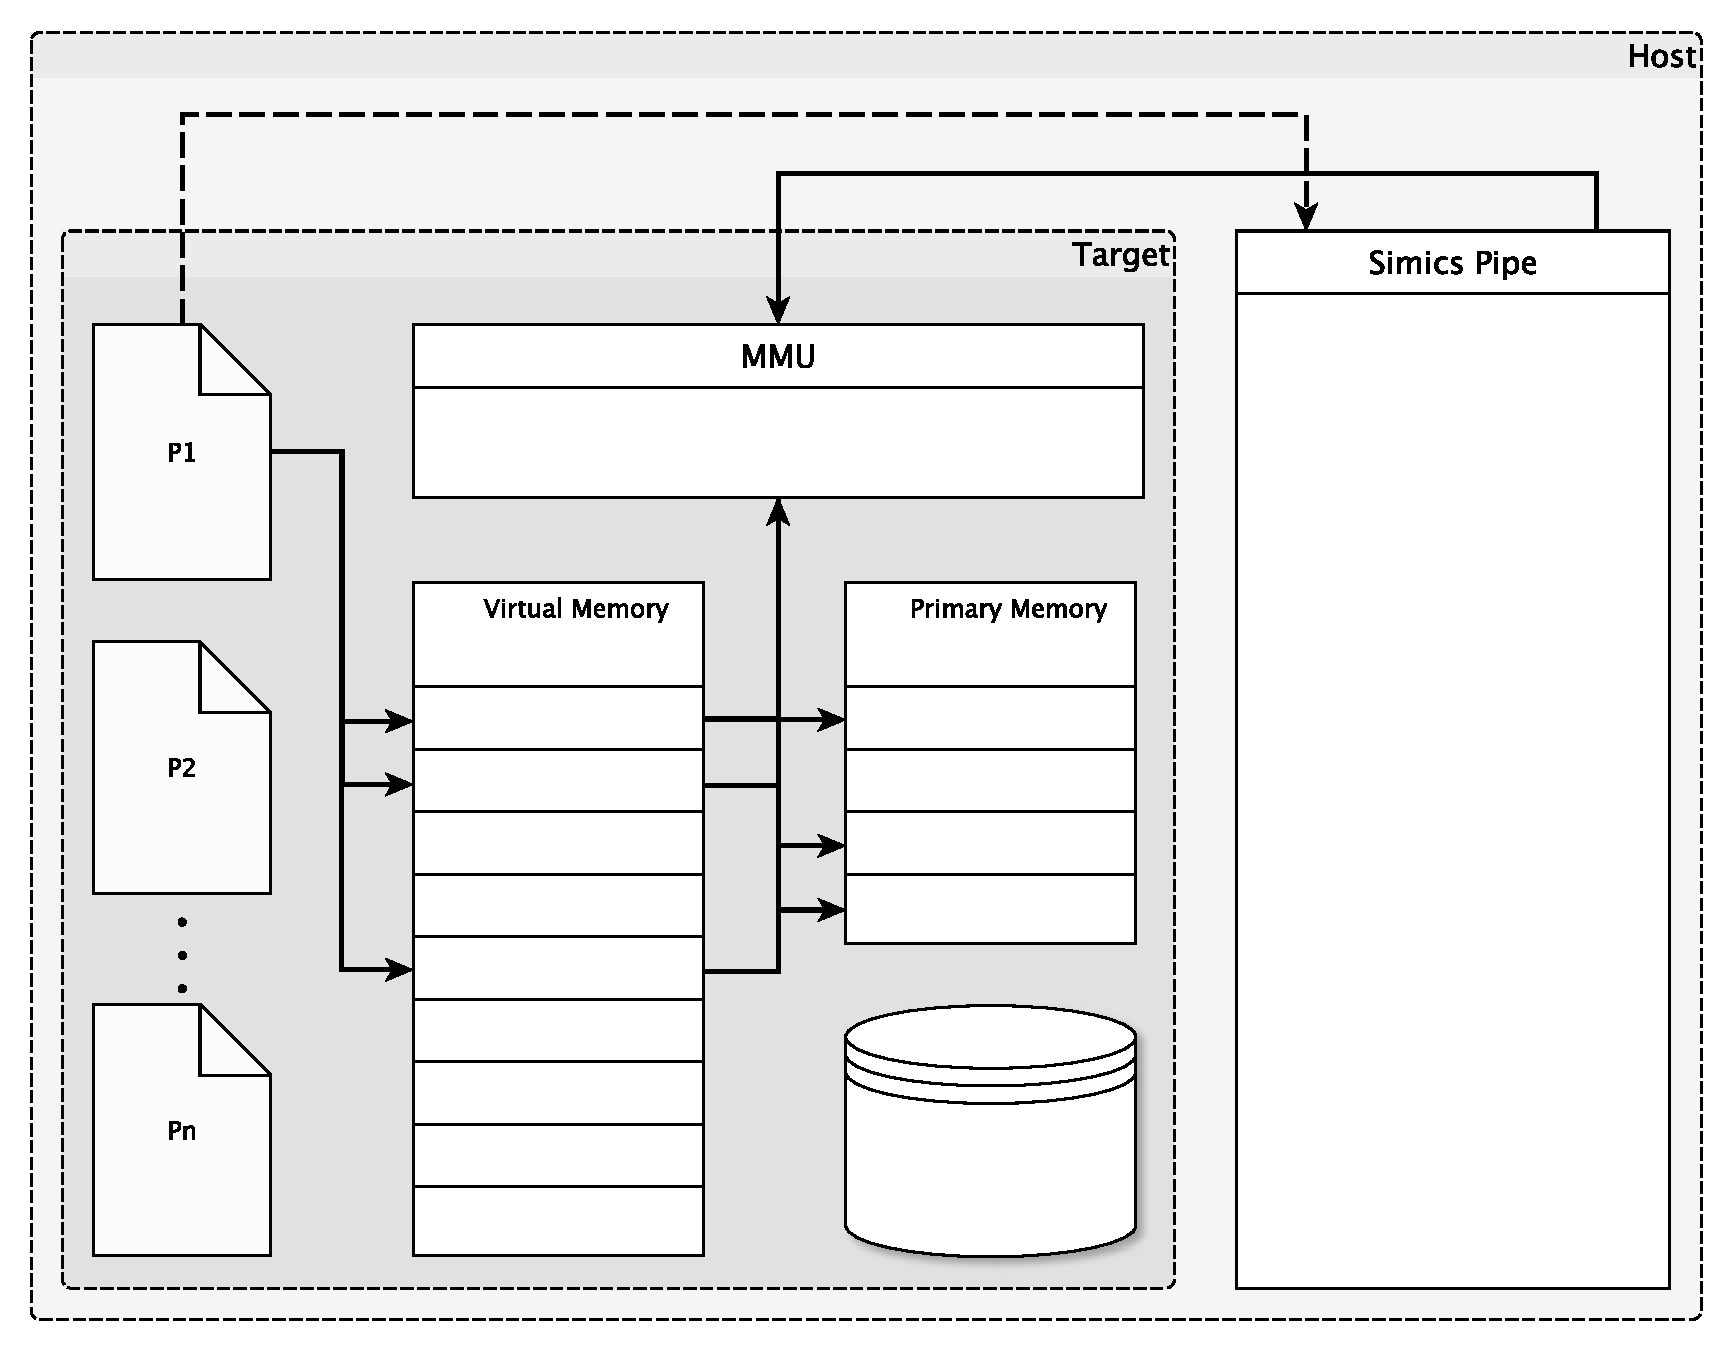
\includegraphics[height=0.8\textheight]{yedvirtualmemory.pdf}
\end{center}

\end{frame}

%% Memory translation overview. The OpenGL process hands a virtual memory
%% address, pointing somewhere in the target system \textit{primary}
%% memory, to the paravirtualized solution - which inquiries the target
%% system MMU to retrieve designated bytestream directly from target
%% physical memory.


        \subsection{Benchmarks}
	\begin{frame}
\frametitle{Benchmarks}

\begin{columns}
  \column{0.5\textwidth}

  \begin{block}{Chess}
    \begin{itemize}
    \item Many lightweight draw calls
    \item Induces many magic instructions, stresses communication latency
    \end{itemize}
  \end{block}

  \begin{block}{Julia}
    \begin{itemize}
    \item Heavy-duty shader
    \item Renders Julia fractal
    \end{itemize}
  \end{block}

  $10$ to $20$ ms per frame on host; $16$ ms frame time $\approx60$ FPS
  
  \column{0.5\textwidth}

  \includegraphics[width=0.45\linewidth]{imgchess.png}
  \hspace{0.2cm}
  \includegraphics[width=0.45\linewidth]{imgjulia.png}

\end{columns}
	
\end{frame}


        \subsection{Results}
        \begin{frame}
  \frametitle{Results - Chess}

  \begin{table}[]
    \centering
    \begin{tabular}{lllll}
      \hline
      Input & \multicolumn{4}{l}{Elapsed time (ms)} \\ \hline
      Tiles & Min & Max & Std & Avg \\
      $60\times60$ & \mascfirstline{simicschess60x60.dat.min} & \mascfirstline{simicschess60x60.dat.max} & \mascfirstline{simicschess60x60.dat.std} & \textbf{\mascfirstline{simicschess60x60.dat.avg}} \\
      $84\times84$ & \mascfirstline{simicschess84x84.dat.min} & \mascfirstline{simicschess84x84.dat.max} & \mascfirstline{simicschess84x84.dat.std} & \textbf{\mascfirstline{simicschess84x84.dat.avg}} \\
      $118\times118$ & \mascfirstline{simicschess118x118.dat.min} & \mascfirstline{simicschess118x118.dat.max} & \mascfirstline{simicschess118x118.dat.std} & \textbf{\mascfirstline{simicschess118x118.dat.avg}} \\ \hline
    \end{tabular}
    \caption{Software rasterization}
  \end{table}

  \begin{table}[]
    \centering
    \begin{tabular}{lllll}
      \hline
      Input & \multicolumn{4}{l}{Elapsed time (ms)} \\ \hline
      Tiles & Min & Max & Std & Avg \\
      $60\times60$ & \mascfirstline{parachess60x60.dat.min} & \mascfirstline{parachess60x60.dat.max} & \mascfirstline{parachess60x60.dat.std} & \textbf{\mascfirstline{parachess60x60.dat.avg}} \\
      $84\times84$ & \mascfirstline{parachess84x84.dat.min} & \mascfirstline{parachess84x84.dat.max} & \mascfirstline{parachess84x84.dat.std} & \textbf{\mascfirstline{parachess84x84.dat.avg}} \\
      $118\times118$ & \mascfirstline{parachess118x118.dat.min} & \mascfirstline{parachess118x118.dat.max} & \mascfirstline{parachess118x118.dat.std} & \textbf{\mascfirstline{parachess118x118.dat.avg}} \\ \hline
    \end{tabular}
    \caption{Paravirtualization}
  \end{table}

\end{frame}

    %% \begin{table}
    %%   \resizebox{0.95\columnwidth}{!}{%
    %%   \begin{tabular}{|c|c|r|r|r|r|}
    %%     \hline
    %%     \multirow{2}{*}{Benchmark} & \multirow{2}{*}{Input} & \multicolumn{4}{p{4cm}|}{\centering Elapsed time (\milli\second )} \\
    %%     \cline{3-6} && \multicolumn{1}{c|}{Min} & \multicolumn{1}{c|}{Max} & \multicolumn{1}{c|}{Std} & \multicolumn{1}{c|}{Avg} \\ \hline
    %%     \multirow{3}{*}{Chess} & \chesskeyone & \mascfirstline{parachess60x60.dat.min} & \mascfirstline{parachess60x60.dat.max} & \mascfirstline{parachess60x60.dat.std} & \textbf{\mascfirstline{parachess60x60.dat.avg}} \\
    %%     & \chesskeytwo & \mascfirstline{parachess84x84.dat.min} & \mascfirstline{parachess84x84.dat.max} & \mascfirstline{parachess84x84.dat.std} & \textbf{\mascfirstline{parachess84x84.dat.avg}} \\
    %%     & \chesskeythree & \mascfirstline{parachess118x118.dat.min} & \mascfirstline{parachess118x118.dat.max} & \mascfirstline{parachess118x118.dat.std} & \textbf{\mascfirstline{parachess118x118.dat.avg}} \\ \hline
    %%     \multirow{3}{*}{Julia} & \juliakeyone & \mascfirstline{parajulia225.dat.min} & \mascfirstline{parajulia225.dat.max}	& \mascfirstline{parajulia225.dat.std} & \textbf{\mascfirstline{parajulia225.dat.avg}} \\
    %%     & \juliakeytwo & \mascfirstline{parajulia450.dat.min} & \mascfirstline{parajulia450.dat.max} & \mascfirstline{parajulia450.dat.std} & \textbf{\mascfirstline{parajulia450.dat.avg}} \\
    %%     & \juliakeythree & \mascfirstline{parajulia900.dat.min} & \mascfirstline{parajulia900.dat.max} & \mascfirstline{parajulia900.dat.std} & \textbf{\mascfirstline{parajulia900.dat.avg}} \\ \hline
    %%   \end{tabular}
    %%   }
    %%   \caption{Paravirtualization}
    %% \end{table}

        \begin{frame}
  \frametitle{Results - Julia}

  \begin{table}[]
    \centering
    \begin{tabular}{lllll}
      \hline
      Input & \multicolumn{4}{l}{Elapsed time (ms)} \\ \hline
      Iterations & Min & Max & Std & Avg \\
      $225$ & \mascfirstline{simicsjulia225.dat.min} & \mascfirstline{simicsjulia225.dat.max} & \mascfirstline{simicsjulia225.dat.std} & \textbf{\mascfirstline{simicsjulia225.dat.avg}} \\
      $450$ & \mascfirstline{simicsjulia450.dat.min} & \mascfirstline{simicsjulia450.dat.max} & \mascfirstline{simicsjulia450.dat.std} & \textbf{\mascfirstline{simicsjulia450.dat.avg}} \\
      $900$ & \mascfirstline{simicsjulia900.dat.min} & \mascfirstline{simicsjulia900.dat.max} & \mascfirstline{simicsjulia900.dat.std} & \textbf{\mascfirstline{simicsjulia900.dat.avg}} \\ \hline
    \end{tabular}
    \caption{Software rasterization}
  \end{table}

  \begin{table}[]
    \centering
    \begin{tabular}{lllll}
      \hline
      Input & \multicolumn{4}{l}{Elapsed time (ms)} \\ \hline
      Iterations & Min & Max & Std & Avg \\
      $225$ & \mascfirstline{parajulia225.dat.min} & \mascfirstline{parajulia225.dat.max} & \mascfirstline{parajulia225.dat.std} & \textbf{\mascfirstline{parajulia225.dat.avg}} \\
      $450$ & \mascfirstline{parajulia450.dat.min} & \mascfirstline{parajulia450.dat.max} & \mascfirstline{parajulia450.dat.std} & \textbf{\mascfirstline{parajulia450.dat.avg}} \\
      $900$ & \mascfirstline{parajulia900.dat.min} & \mascfirstline{parajulia900.dat.max} & \mascfirstline{parajulia900.dat.std} & \textbf{\mascfirstline{parajulia900.dat.avg}} \\ \hline
    \end{tabular}
    \caption{Paravirtualization}
  \end{table}

  \begin{itemize}
  \item Software rasterization very slow
  \item Paravirtualization drastically reduce the performance hit
  \item Improvements of up to $34$ times
  \end{itemize}

\end{frame}


        \subsection{Hardware-assisted virtualization}
        \begin{frame}
\frametitle{Hardware-assisted virtualization}

\begin{table}[]
\centering
\caption{Chess - approximately one order of magnitude}
\begin{tabular}{ll}
\hline
Paravirtualization & Software Rasterization \\ \hline
$\approx 1$ sec. & $\approx 7$ sec. \\
$\approx 2$ sec. & $\approx 10$ sec. \\
$\approx 3$ sec. & $\approx 13$ sec. \\ \hline
\end{tabular}
\end{table}

\begin{table}[]
\centering
\caption{Julia - up to three orders of magnitude}
\begin{tabular}{lll}
\hline
Paravirtualization & Software Rasterization \\ \hline
$<\frac{1}{10}$ sec. & $\approx 1$ min. \\
$<\frac{1}{10}$ sec. & $<2$ min. \\
$\approx \frac{1}{10}$ sec. & $\approx 3$ min. \\ \hline
\end{tabular}
\end{table}

%% \begin{itemize}
%% 	\item Without hardware-assisted virtualization, hit to software rasterization is roughly two orders of magnitude compared to hardware acceleration
%% 	\item Hit to paravirtualization is often less than an order of magnitude
%% 	\item Paravirtualization renders up to three orders of magnitude faster than software rasterization
%%         \item This entails that the Chess benchmark is accelerated by paravirtualization
%%         \item We conclude that effects of paravirtualization increase by one order of magnitude if hardware-assisted virtualization is not available
%%         \item Workloads that are otherwise sub-optimal are thus accelerated
%% \end{itemize}

\end{frame}


        \section{Conclusion}

        \subsection{Future work}
	\begin{frame}

\frametitle{Future work}

\begin{itemize}
  \item Command serialization batching \begin{itemize}\item WireGL\end{itemize}
  \item Extending supported frameworks \begin{itemize}\item DirectX $\rightarrow$ OpenGL\end{itemize}
  \item General purpose, GPGPU \begin{itemize}\item OpenCL\end{itemize}
\end{itemize}

\end{frame}


        \subsection{Recap}
	\begin{frame}
\frametitle{Recap}

\begin{block}{\#1}
	Paravirtualization is a viable method to accelerate graphics
\end{block}

\begin{block}{\#2}
	Magic instructions are fit for purpose
\end{block}

\begin{block}{\#3}
	The case for paravirtualization is strengthened for systems where hardware-assisted virtualization is unavailable
\end{block}

\end{frame}


        \begin{frame}
  Authors:

  \begin{columns}
    \column{0.5\textwidth}
    \begin{itemize}
    \item Eric Nilsson
    \item Daniel Aarno
    \end{itemize}
    \column{0.5\textwidth}
    \begin{itemize}
    \item Erik Carstensen
    \item H{\aa}kan Grahn
    \end{itemize}
  \end{columns}

  \vspace{1cm}

  \begin{center}
    \url{http://www.windriver.com/products/simics/}
  \end{center}

  \vspace{1cm}

  \begin{center}\tiny
    Wind River is a trademark or registered trademark of Wind River Systems Inc. and its affiliates.

    Intel and the Intel logo are trademarks of Intel Corporation in the U.S. and/or other countries.

    Other names and brands may be claimed as the property of others.
  \end{center}

\end{frame}


        % Appendix
        % fig:histogram
\begin{figure}
  \setlength{\abovecaptionskip}{-5pt}
  \setlength{\belowcaptionskip}{0pt}
  \centering
  \input{gnuhistogramssimicsparachess.tex}
  \input{gnuhistogramssimicsparajulia.tex}
  \caption{Sample histograms depicting $1000$ frames subdivided into $100$ bins, presented in milliseconds. Top $2\times3$: Chess. Bottom $2\times3$: Julia.}
  \label{fig:histogram}
\end{figure}

\end{document}
